\chapter{Konputazio zientzia.}

%\epigraph{Optimizing a program can be a better solution than buying a faster computer!}
%{\textit {Performance optimization of Numerically Intensive Codes(2001)}}

\section{Sarrera.}

Azken hamarkadetan,  konputazio zientziaren hazkundea oso handia izan da eta bere erabilera ia zientzia arlo guztietara zabaldu da \cite{Goedecker2001}. Zientzialariek ahalmen handiko tresna berria (zenbakizko simulazioa) eskuragarri dute, neurri handi batean konputagailuen teknologiaren garapen handiari esker. Egungo oinarrizko konputagailuek, orain urte gutxitako superordenagailuen ahalmen berdina dute eta superordenagailuen konputazio gaitasuna ere, maila berdinean hazi da. Zenbakizko algoritmoek ere, garapen handia izan dute; algoritmo eraginkorragoak, idei berriak sortuz eta konputagailuen gaitasunei egokituz, garatu dira.

Konputazioaren alde garestiena, memoria eta prozesadorearen arteko datu mugimendua da. Prozesadoreak gero eta azkarragoak dira, baina memori atzipenaren abiaduraren hobekuntza mugatuagoa dago. Horregatik algoritmo eraginkorrak, prozesadorearen konputazio arik eta handiena,  memoria komunikazio arik eta txikienarekin, diseinatu behar dira.      
 
Inplementazio baten eraginkortasuna ez da exekuzio denboraren arabera bakarrik neurtu behar. Hori bezain garrantzitsua da kode ona idaztea \cite{Wilson2014} eta zentzu honetan hiru ezaugarri hauek bereziki zaindu behar dira:
\begin{enumerate}
\item Errorerik gabeko kodea.
\item Kode argia idaztea.
\item Etorkizunean erraz aldatu daitekeen kodea.
\end{enumerate}

Kapitulu honetan,  konputazio zientziaren funtsezko osagaiak azalduko ditugu. Lehenengo, konputazioaren eraginkortasuna aztertzeko eta exekuzioak neurtzeko tresnen zehaztapenak emango ditugu. Ondoren, konputagailu hardware berriak eta paralelizazio gaitasunak laburtu dugu. Jarraian software ikuspegitik, programazio lengoaiak eta aljebra linealerako (LAPACK) liburutegia landu dugu. Azkenik, konpiladoreari buruzko argibide batzuk eman ditugu.

\section{Eraginkortasuna}

Konputazio zientziaren inplementazio berri baten eraginkortasuna neurtzeko, koma-higikorreko eragiketa kopurua (\emph{flops}) erabili ohi da. Problema handia denean, datuen mugimendua koma-higikorreko eragiketak baino garestiagoa da eta eraginkortasuna, eragiketa kopuruaren arabera neurtzea okerra izan daiteke. 

Prozesadoreen maiztasun-abiadura hertzetan neurtzen da, hau da,  \emph{makina ziklo segundoko} kopuruaren arabera. Une honetako prozesadoreak gigahertz (Giga = $10^9$) mailakoak dira. Koma-higikorreko oinarrizko eragiketa bat ($\oplus,\ominus,\otimes,\oslash$) exekutatzeko  ziklo gutxi batzuk behar dira eta beraz, $1$ GHz-ko prozesadore batek
$>10^8$ koma-higikorreko eragiketa segundoko exekutatzen ditu ($>100$ megaflops) \cite{Pacheco2011}.

\paragraph*{\textbf{Adibidea}.} 
Demagun $A,B$ eta $C \ (n \times n)$ dimentsioko matrizeak ditugula eta $C=AB$ matrize arteko biderketa egiteko behar dugun denbora jakin nahi dugula.
\begin{equation*}
c_{ij}=\sum\limits_{i,j=1}^{n} a_{ij}*b_{ji}.
\end{equation*}

\begin{itemize}
\item $c_{ij}$ gai bakoitza kalkulatzeko $n$ biderketa eta ($n-1$) batura egin behar ditugu.
\item $C$ matrizeak $n^2$ osagaia ditu $\Rightarrow$ $\mathcal{O}(n^3)$ koma-higikorreko ariketak exekutatu behar dira.
\end{itemize}

Matrizearen tamaina $n=100$ bada,  orduan  $\mathcal{O}(n^3)=10^{6}$ eragiketa egin behar ditugu. $1$-GHz prozesadore batean exekutatzeko, $10^{-2}$ segundo baino gehiago beharko genituzke. Baina matrize honek,  $3.9$ \emph{MB} memoria beharrezkoa du eta  konputagailuaren Cache memoria baino handiagoa dela suposatuz, exekuzio denboran datuen mugimenduaren eragina nabarmena izango da. 

Konputazio gaitasuna (\emph{peak}), hardwareak fisikoki exekutatu dezakeen eragiketa kopuru maximoa bada, aplikazio gehienak, konputagailuaren konputazio gaitasunaren  $\%10$ baino gutxiagorekin exekutatzen dira.  Eraginkortasun horren txikia, memoria irakurketa/idazketetan galtzen da. Azpimarratu nahi dugu, $t_f$ eragiketa aritmetiko bat egiteko denbora bada eta $t_m$, datu bat memoria nagusitik cache memoriara mugitzeko denbora bada,
\begin{equation*}
 t_f \ll t_m,
\end{equation*}
eta etorkizunean, diferentzia hau handituz joango dela. Beraz, kodearen exekuzioa azkartzeko derrigorrezkoa da konputagailuan memorien arteko datuen mugimendua minimizatzea.
       
\subsubsection*{Exekuzio denboren neurketa.}

Unix-eko \emph{time} agindua, konputazioen denborak ezagutzeko erabili daiteke \cite{Pacheco2011}:

\begin{lstlisting} 
S time ./a.out
<kodearen irteera>

real 0m38.856s
user 0m38.789s
sys  0m0.004s
\end{lstlisting}

Agindu honek, \emph{./a.out} C programa exekutatuko da eta ondoren, programa exekutatzeko behar izan duen denboraren informazioa pantailaratuko du:
\begin{itemize}
\item  \emph{real}: hasi eta bukatu arteko denbora (\emph{wall-time} edo \emph{elapsed-time}).
\item \emph{user}:  prozesadoreak gure programa exekutatzen erabili duen denbora (\emph{CPU-time}).
\item \emph{sys}:  programa exekutatu ahal izateko, sistema eragile lanetan emandako denbora. 
\end{itemize}

Programa osoaren konputazio denborak ezagutu beharrean, kodearen zati bat neurtu nahi dugunean, C lengoaiaren bi funtzio hauek erabilgarriak ditugu:

\begin{enumerate}
\item clock().

Funtzioaren bi deien arteko CPU denbora neurtzeko erabiliko dugu (\textbf{CPU time}).

\begin{lstlisting}[language=C]

#include <time.h>

    clock_t clock0, clock1; 
    double elapsed_cpu_time;

    clock0= clock();

    <neurtu nahi den kodea>

    clock1=clock();
    
    elapsed_cpu_time=(clock1 - clock0)/CLOCKS_PER_SEC);

\end{lstlisting}

\item time().

Funtzioaren bi deien artean igarotako denbora neurtzeko erabiliko dugu (\textbf{elapsed-time}).

\begin{lstlisting}[language=C]

#include <time.h>

    time_t  time0,time1;
    double elapsed_time;

    time(&time0);

    <neurtu nahi den kodea>

    time(&time0);
    
    elapsed_time=difftime(time1,time0);

\end{lstlisting}

\end{enumerate}

CPU denborari buruzko argibide bat ematea komeni da. Neurtzen ari garen kodea sekuentzialki exekutatzen bada, hau da, hari (\emph{thread}) bakarrekoa, orduan kode zati hori exekutatzeko erabili duen CPU denbora itzuliko du. Aldiz, kodea paraleloan exekutatzen bada, orduan , hari guztien CPU denboren batura itzuliko ditu. 


\paragraph*{Adibidea.} Argiago azaltzeko, $C=AB$ matrize biderketaren kodearen bi exekuzioen denboren neurketak zehaztuko ditugu:

\begin{enumerate}
\item $200 \times 200$ tamainako, bi matrizeen biderketa sekuentzialaren denborak hauek izan dira:
\begin{lstlisting}
elapsed-time=2.1s
elapsed-cpu-time=2.07s
\end{lstlisting}

\item $200 \times 200$ tamainako, bi matrizeen biderketa paraleloaren (hariak=$2$) denborak hauek izan dira:
\begin{lstlisting}
elapsed-time=1.0s
elapsed-cpu-time=2.35s
\end{lstlisting}
 
 
\end{enumerate}
 
\emph{Elapsed-time} deiturikoa, kode paraleloen denborak neurtzeko irizpidea da. Programazio paraleloan, algoritmoen exekuzio denborak egokien neurtzen duen aldagaia da baina, une berean programa bakarra exekutatzea behartuta gaude.       


\section{Hardwarea.}


Orokorrean, gaur-egungo konputagailuak (super-konputagailu, eramangarri,...) paraleloak dira. $1986-2002$ urteen artean, txip barruko transistore dentsitatea handitzen zen heinean, prozesadore bakarreko konputagailuen eraginkortasuna hobetuz joan zen. Baina teknologi honen garapena muga fisikoetara iritsi zenean, bide honetatik konputagailuen abiadura hobetzea ezinezkoa bilakatu zen. Horrela, 2005.urtetik aurrera fabrikatzaileek konputagailuen gaitasuna hobetzeko, txipan prozesadore bat baino gehiago erabiltzea erabaki zuten.  

%\begin{itemize}
%\item Moore's Law (1965). Processor speed doubles every 18 months.
%\item Moore's Law Reinterpreter (2006). Number of cores per chip can double every two years.
%\end{itemize}    

Konputagailuen eredu aldaketa honen ondorioz, algoritmo azkarrak garatzeko kodearen paralelizazio gaitasunari heldu behar zaio. Programazio paralelo teknikak inplementatzeko, beharrezko da prozesadore berrien hardware arkitektura berriak ulertzea. Gaia nahiko konplexua izanik, ikuspegi orokor bat ematera mugatuko gara. \ref{fig:IntelXeon}~irudian ikusi daitekeenez, Intel Xeon konputagailu familiaren paralelizazio eta bektorizazio gaitasuna gero eta handiagoak dira.  


\begin{figure}[h]
{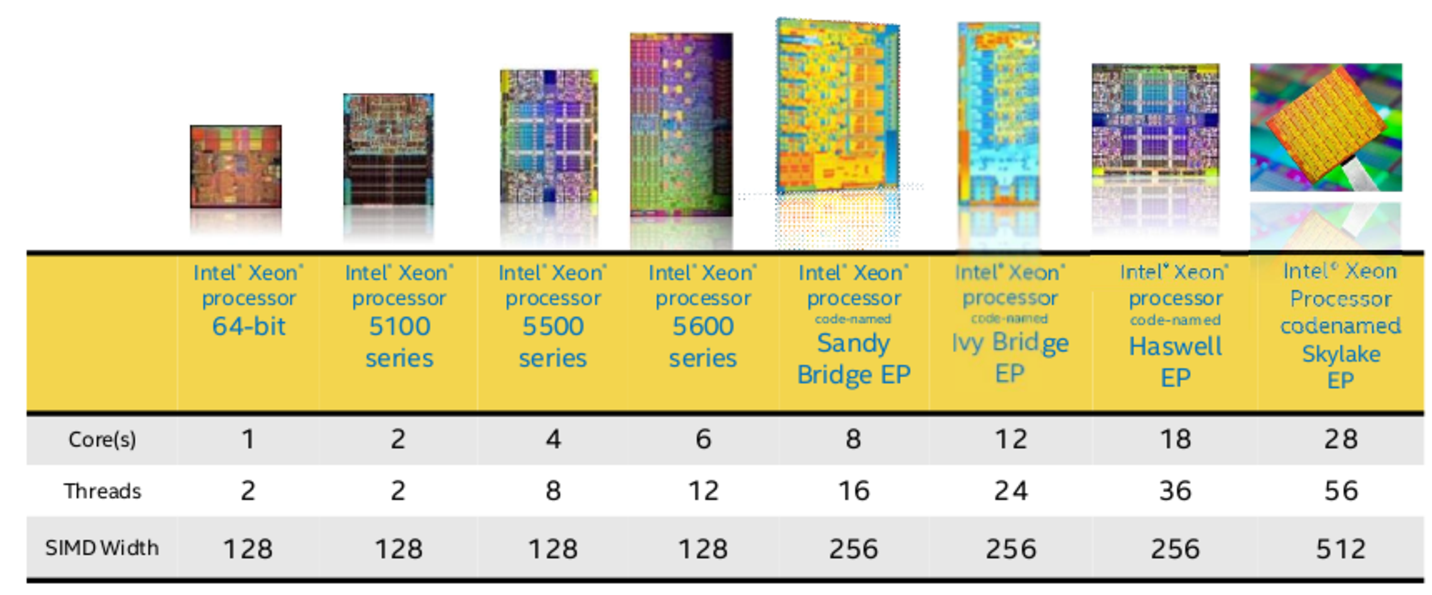
\includegraphics[width=14cm, height=6cm] {IntelXeonSeries}}
\caption[Intel Xeon konputagailuak]{Intel Xeon konputagailu familiaren eboluzioa: gero eta prozesadore gehiago eta bektore erregistro zabalagoak.}
\label{fig:IntelXeon}
\end{figure} 


\subsection*{Memori hierarkia.}

Memorien arteko datuen komunikazioak, algoritmoaren eraginkortasuna baldintzatuko du eta zentzu honetan, konputagailuaren memoria hierarkiaren kudeaketa egokia egitea funtsezkoa da. Konputagailuaren memoria mota ezberdinen hierarkia (\ref{fig:memhier}irudia) eta funtzionamendua deskribatuko dugu. 
\begin{figure}[h]
\centerline{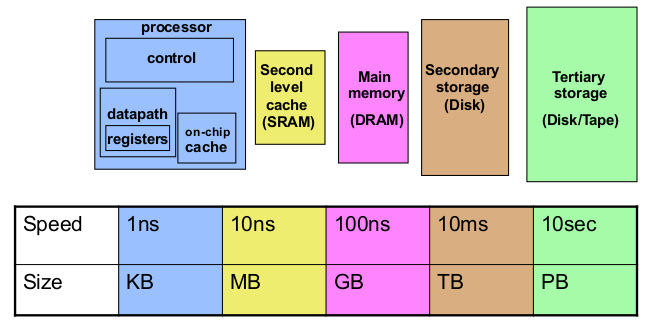
\includegraphics[width=10cm, height=4cm] {MemoryHierarchy}}
\caption[Memoria hierarkia]{Memoria hierarkia.}
\label{fig:memhier}
\end{figure} 

CPU-k, koma-higikorreko eragiketak exekutatzen ditu: erregistroetatik datuak irakurri, eragiketak kalkulatu eta emaitza erregistroetan idazten ditu. Memoria nagusia eta erregistroen artean, $2$ edo $3$ mailako cache memoria dugu: lehen cache memoria ($L1$) txikiena eta azkarrena da, eta beste mailak ($L2$, $L3$,\dots), handiagoak eta motelagoak dira. Memoria nagusian, exekutatzen diren programak eta datuak gordetzen dira ($1-4$ GB artekoa). Azkenik, disko gogorrean konputagailuko datu (argazki, bideo,...) eta erabilgarri ditugun programa guztiak gordetzen dira.  

CPU-k datu bat behar duenean, memoria hierarkian zehar bilatuko du: lehenik $L1$ cachean, ondoren $L2$ cachean,...eta hauetan ez badago, memoria nagusira joko du. Memoria nagusi eta cache memoria arteko irakurketa eta idazketa guzti hauetan,  informazio kontsistentea mantentzeko hainbat arau aurrera ematen dira. 

Cache memoria lerroka egituratuta dago eta lerro bakoitza $64$ edo $128$ bytez ($8$ edo $16$ doitasun bikoitzeko zenbaki) osatuta dago. Programa batek datu bat behar duenean, memoria nagusitik lerro tamainako datu taldea (memorian jarraian gordetako datuak) irakurriko du eta cachean idatziko du. Programatzaileak, algoritmo eraginkorrak inplementatzeko memorien arteko komunikazio hau minimizatzen saiatu behar du eta horretarako, inplementazioaren diseinua datuen memoria atzipen jarraian oinarritu behar du. Ezaugarri hau, \emph{spatial/data locality} izenaz ezaguna da eta helburua, cachera ekartzen diren datuak, memoria nagusian idatzi aurretik gutxienez behin erabiltzea da. 

\paragraph*{Adibidea.} Adibide honetan, $A=(a_{ij})_{i,j}^{n,m}$ matrize baten osagaien batura ($sum=\sum_{i,j=0}^{n,m} a_{ij}$) kalkulatzeko bi inplementazio aztertuko ditugu. C lengoaian matrizeak lerroka gordetzen dira ($n=m=100$),
\begin{equation*}
A=\left(\begin{array}{ccccc}
  1    & 2    & 3    & \dots & 100 \\
  101 & 102 & 103 &\dots & 200 \\
  201 & 202 & 203 &\dots & 300 \\
  \dots & \dots & \dots & \dots & \dots \\
  9.901 & 9.902 & 9.903 &\dots & 10.000 \\
  \end{array}\right).  
\end{equation*}
eta horregatik, lehen aukera bigarrena baino eraginkorragoa izango da. Lehen inplementazioan, kanpo iterazioa lerroka (Algoritmoa \ref{algo:lerroka}):  matrizearen lehen osagaia $a(1,1)$ behar dugunean, memoria nagusitik Cachera osagai honetaz gain, jarraiko 16 osagaiak ekarriko dira ($a(1,1),a(1,2),\dots,a(1,16)$). Honela, hurrengo $15$ batura egiteko behar ditugun datuak Cachean eskura izango ditugu memoria irakurketa berririk egin gabe. Bigarren inplementazioan, kanpo iterazioa zutabeka (Algoritmoa \ref{algo:zutabeka}): bigarren osagaia ($a(2,1)$) gehitzeko memoria irakurketa berri bat egin behar dugu. 

\begin{algorithm}[h]
 \BlankLine
  $int \ n$\;
  $double \ a[n][m]$\;
  \BlankLine
  $sum=0$\;
  \For{$i\leftarrow 1$ \KwTo $n$}
  {
   \BlankLine
    \For{$j\leftarrow 1$ \KwTo $m$}
   {
    \BlankLine 
    $sum+=a(i,j)$\;
   }
 }
 \caption{Memoria atzipena eraginkorra.}
 \label{algo:lerroka}
\end{algorithm} 
\begin{algorithm}[h]
 \BlankLine
  $int \ n$\;
  $double \ a[n][m]$\;
  \BlankLine
  $sum=0$\;
  \For{$j\leftarrow 1$ \KwTo $m$}
  {
   \BlankLine
    \For{$i\leftarrow 1$ \KwTo $n$}
   {
    \BlankLine 
    $sum+=a(i,j)$\;
   }
 }
 \caption{Memoria atzipena ez-eraginkorra.}
 \label{algo:zutabeka}
\end{algorithm} 


\subsection*{Arkitektura motak.}

Prozesadore anitzeko konputagailu hardware berriak, konplexuak eta heterogeneoak dira. Egoera honetan, programatzaileak zailtasun handiak ditu arkitektura berriek eskaintzen dituzten gaitasunak ondo kudeatzeko \cite{Luszczek2014}.   

Lehen hurbilpen modura bi sistema nagusi bereiziko ditugu:  memoria konpartitutako eta memoria banatutako sistemak. Memoria konpartitutako sistemetan, prozesadore guztiek memoria osoa konpartitzen dute eta inplizituki konpartitutako datuen atzipenaren bidez komunikatzen dira (\ref{fig:mks} irudia). Memoria banatutakotako sistemetan aldiz, prozesadore bakoitzak bere memoria pribatua du eta esplizituki bidalitako mezuen bidez komunikatzen dira (\ref{fig:mbs} irudia). Aipatzekoa da, sistema handietan bi memoria motak nahasten direla, hau da, batetik goiko mailan memoria banatuta alde bat eta bestetik, konputazio unitate bakoitzak memoria konpartitutako aldea.    

Hirugarren sistema osagarria ere aipatuko dugu, GPU (Graphical Processor Unit) unitateetan oinarritutako konputazioa.
Jokoen eta animazio industrian, grafiko oso azkarrak beharrak bultzatuta  sortutako teknologia da. Oinarrian, imajinak pantailaratzeko prozesagailu asko paraleloan lan egiten dute eta azken hamarkadan, \emph{GPU} unitate hauek  konputazio zientziara zabaldu dira.  

\begin{figure}[h]
\centerline{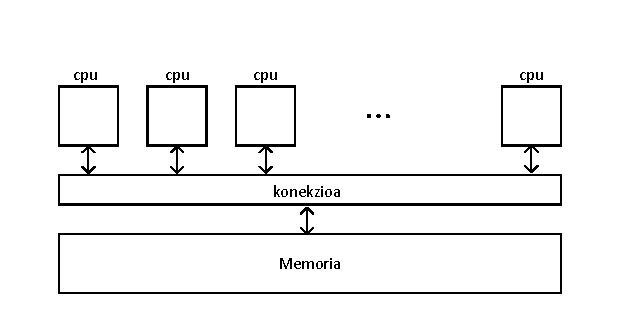
\includegraphics[width=12cm, height=6cm] {Arkitektura1}}
\caption[Memoria konpartitutako sistemak]{Memoria konpartitutako sistemak}
\label{fig:mks}
\end{figure}  

\begin{figure}[h]
\centerline{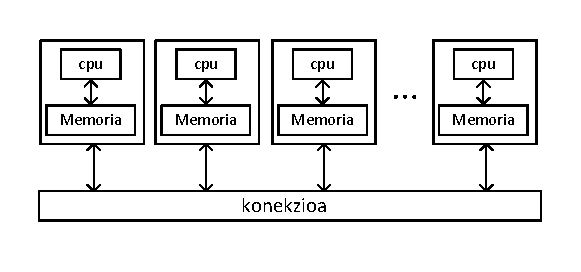
\includegraphics[width=12cm, height=4cm] {Arkitektura2}}
\caption[Memoria banatutako sistemak]{Memoria banatutako sistemak}
\label{fig:mbs}
\end{figure}  

\subsubsection*{Oinarrizko konputagailu paraleloa.}

Gure lanerako, oinarrizko konputagailu paraleloak kontsideratuko ditugu: memoria konpartitutako eta prozesadore anitzeko unitate bat edo gehiagoz osatutako sistemak. Prozesadore anitzeko unitate bakoitzak txipean CPU bat baino gehiago ditu. Normalean CPU bakoitzak $L1$ bere cache memoria du. Aipatzeko da, era honetako sistemetan prozesadore kopurua mugatua dela (normalean $\leq 32$ ) \cite{Pacheco2011,EijkhoutHPC}.

Memoria konpartitutako sistemen artean bi mota bereiziko ditugu:

\begin{enumerate}
\item UMA sistemak (uniform memory access). 
Txip prozesadore guztiak zuzenean memoria konektatuta daude eta guztiak atzipen denbora berdina dute (\ref{fig:UMA}.irudia).

\begin{figure}[h]
 \centerline{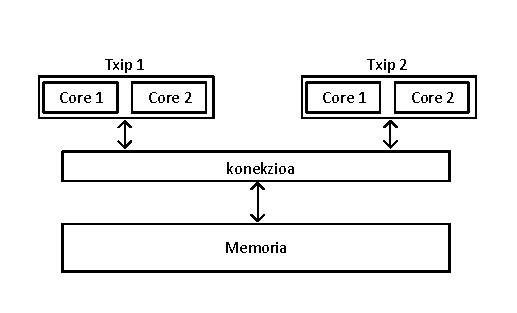
\includegraphics[width=12cm, height=5cm] {ArkitekturaUMA}}
 \caption[UMA sistemak]{Memoria konpartitutako sistemak (UMA).}
 \label{fig:UMA}
\end{figure}  

\item NUMA sistemak (nonuniform memory access).
Txip prozesadore bakoitza, hardware berezi baten bidez zuzenean memoria bloke bati konektatuta dago. Zuzenean konektatuta dagoen memori blokearen atzipen denbora, beste txipan zehar konektatutako memoriaren atzipena baina azkarragoa da ( \ref{fig:NUMA}.irudia).

\begin{figure}[h]
 \centerline{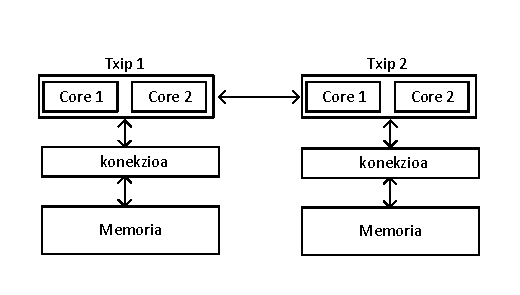
\includegraphics[width=12cm, height=4cm] {ArkitekturaNUMA}}
 \caption[NUMA sistemak]{Memoria konpartitutako sistemak (NUMA).}
 \label{fig:NUMA}
 \end{figure}  
\end{enumerate}  

\subsubsection*{Bektorizazioa (SIMD).}

Prozesadore berriei hardware bektore unitateak gehitu zaizkie, eta  (AVX) bektore instrukzioetan oinarritutako paralelizazioa eskaintzen dute \cite{Muller2009,Andrey2013}. CPU-ak bektore erregistroan gorde diren zenbaki multzo bati, eragiketa berdina aplikatzen die (\emph{Single Instruction Multiple Data}, SIMD). Bektore erregistro hauek  $512$-biteko tamainakoak ($512/64=8$ doitasun bikoitzeko zenbaki) izan daitezke eta oro har, oinarrizko eragiketa aritmetikoak (batuketa, kenketa, biderketa eta zatiketa) aplika daitezke. Zentzu honetan ulertu behar da hardware bidezko bektorizazioak,  doitasun bikoitzeko konputazioen eraginkortasuna $x8$ hobetzen duela  eta doitasun arrunteko konputazioetan, berriz, $x16$.     

Adibide moduan, hurrengo adibidearen bidez, iterazio bakoitzean 8 osagaien bektore baten batura erakutsiko nahi dugu,

\begin{algorithm}[H]
 \BlankLine
  \For{$i=0$; $i<n$ ; $i+=8$}
  {
   \BlankLine
    $A[i:(i+8)]=A[i:(i+8)]+B[i:(i+8)]$\;
   \BlankLine
  }
 \caption{SIMD (bektorizazioa).}
\end{algorithm}


\section{Programazio lengoaiak (Paralelizazioa).}

Fortran eta C, aplikazio zientifikoetan gehien erabiltzen diren programazio lengoaiak dira \cite{Higham2015}. Fortran (formula translation) 1950 hamarkadan garatutako goi-mailako lehen lengoaia izan zen eta oraindik ere, oso zabaldua da. Fortran estandarraren hainbat bertsio 
sortu dira: Fortran 66, 77, 90, 95, 2003 eta 2008. Hauetako bertsio bakoitzean funtzionalitate berriak  eta C lengoaiarekin lan egiteko bateragarritasuna gehitu zaizkio.  C lengoaia, 1970 hamarkadan jaio zen eta hardwarearekiko hurbiltasun" ezaugarri nagusiak, konpiladoreari kode eraginkorra sortzeko aukera ematen dio. C lengoaia \emph{UNIX} sistema eragileari lotuta jaio zen eta hurrengo garapenetan bere izaera askea mantendu du. C lengoaiaren estandarrak 1989, 1999 eta 2011 dira.   

Fortran eta C lengoaiek, ez dituzte kodea paraleloan exekutatzeko tresnarik, hau da, ez dago konputazio banatu, eta prozesadore ezberdinen artean aldi berean exekuzioak zehazteko modurik. Konputazioa paraleloa inplementatzeko, bi dira interfaze aplikazio programa (\emph{API}) moduan inplementatuta dauden sistema nagusiak \cite{Pacheco2011}:

\begin{enumerate}
\item  \emph{MPI} (Message Passing Interface).
Erabiliena da, memoria banatutako sistemetarako pentsatua baina memoria konpartitutako sistemetan ere aplika daitekeena.

\item  \emph{OpenMP} (Open Specifications for MultiProcessing).
Erabiltzeko errazagoa eta memoria konpartitutako sistemetan bakarrik aplika daitekeena.

\end{enumerate}

Errendimendu altuko konputazioaren (\emph{high performance computing}) programazioa konplexua da: espezializazio handikoa  eta konputagailuen hardware jakin baterako egokitutakoa. Zaitasun hauek, proiektu zientifikoak aurrera ateratzeko eta mantentzeko arazo asko eragiten ditu. Azken urteotan, eragozpen hau gainditzeko, programazio lengoaia interesgarriak sortu dira (adibidez, Julia \cite{Bezanson2014} edo Chapel \cite{Balaji2015}) baina oraindik, hauen arrakasta ikustekoa da.

Azkenik,  konputazio zientzian \emph{problemak ebazteko inguruneak} (Problem Solving Enviroments) deituriko softwareak aipatuko ditugu. Ingurune hauek, programazio leiho interaktibo batean, goi-mailako lengoai batean inplementazioen garapena eta emaitzen azterketa egiteko aukera eskaintzen dute. Matlab eta Mathematica \cite{WolframResearch} programazio ingurune nagusienak dira. Guk Mathematica bi modutara erabili dugu. Lehenik, prototipoak garatzeko tresna gisa: idei berriak garatu eta probatu, inplementazioa C lengoaian egin aurretik. Bigarrenik, gure C inplementazioen esperimentuak Mathematica ingurunetik exekutatu eta emaitzak grafikoki aztertu ditugu. Era honetan, irakurleari Mathematicako dokumentuetan esperimentuen zehaztasun guztiak eta esperimentu berdina errepikatzeko aukera ematen diogu.       

\subsection*{OpenMP}   

\emph{OpenMP} \cite{OpenMP} memoria konpartitutako sistemetan programazio paraleloa exekutatzeko interfaze aplikazio programa (\emph{API}) da. \emph{OpenMP} programazioan, memoria osoaren atzipena duten prozesadore multzo batek osatzen du konputazio sistema.

Hasieran programaren hari bakarra prozesadore batean exekutatuko da, kode-paraleloko unera iritsi arte. Orduan, hari multzo independenteak exekutatuko dira une paraleloa bukaera iritsi arte. Exekuzio kontrolari, \emph{fork-join} eredua deitzen zaio eta grafikoki (\ref{fig:forkjoin} irudian ) adierazi dugu.
 
\begin{figure}[h]
\centerline{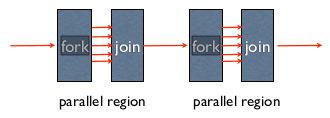
\includegraphics[width=12cm, height=4cm] {ForkJoin}}
\caption[OpenMP programazio modeloa]{OpenMp programazio eredua}
\label{fig:forkjoin}
\end{figure}  
 
\begin{itemize}
\item OpenMP programen hasieran prozesu bakarra dago, hari (thread) nagusia. 
\item FORK: hari nagusiak, hari talde paraleloa sortzen du.
\item JOIN: kode-paraleloko hari guztiak bukatzen dutenean (sinkronizazioa), hari nagusiak soilik jarraitzen du.
 \end{itemize}

Paralelizazioan hari kopurua zehaztu behar da, eta ohikoa izaten da hari bat prozesadore bakoitzeko sortzea. Konpilazio direktiben bidez (C kodean \emph{pragma} izeneko preprozesadore aginduak),  paralelizazioa nola exekutatu behar den zehazten da.
\begin{itemize}
\item Kode paralelizagarria adierazi.
\item Hariaren datu pribatuak zehaztu.
\item Harien arteko sinkronizazioa.
\end{itemize}


\paragraph*{\textbf{Adibidea1.}} C lengoaian, \emph{OpenMP} konpilazio direktibak adierazteko \emph{pragma} hitza lerroaren hasieran idatziko dugu. Adibide honetan, programaren \emph{for-iterazioa} paraleloan exekutatu daitekeela  eta hari kopurua bi dela zehaztu dugu. 

\begin{lstlisting}[language=C]
#    include <omp.h>

     int thread_count=2;

#    pragma omp parallel for num_threads(thread_count) 
     for (i = 0; i<n; i++)
     {
       ! Aginduak 
     }
\end{lstlisting}

Konpilazioan, \emph{-fopenmp} aukera zehaztu behar dugu,
\begin{lstlisting}[language=C]
$ gcc -g -Wall -fopenmp adibidea.c -o adibidea.o.
\end{lstlisting}
Orokorrean, defektuz aldagaia guztiak harien artean konpartituta daude eta aldagaiak pribatuak direla zehazteko, esplizituki adierazi behar da. Goiko adibidea salbuespena da; \emph{for} iterazioaren kontagailua  (adibideko $i$ aldagaia) pribatua da.

Algoritmo batean, kodearen zati bat  da paralelizagarria \cite{Pacheco2011}. Suposa dezagun, konputazioaren $\%50$ sekuentziala dela eta beste $\%50$ paraleloan exekutatu daitekeela. Zati sekuentzialak, lortu daitekeen konputazio optimoena (zati paralelizagarriaren exekuzio denbora zero dela kontsideratzea) mugatuko du eta beraz, gehienez exekuzio sekuentziala baino bi aldiz azkarrago izango da. 
Kontzeptu hau orokortzen badugu, konputazioaren $(1/S)$ sekuentziala eta gainontzekoa, $(1-1/S)$ paralizagarria kontsideratuz, orduan kode optimoena prozesadore kopurua edozein delarik, $S$ faktorea hobea izango da. $T_s$ makina sekuentzial batean exekuzio denbora izendatzen badugu, $P$ prozesadore kopurua erabiliz lortuko den konputazio denbora $T_p$,
\begin{align*}
T_p &=(1/S)T_s + (1-1/S)T_s/P,
\end{align*}
eta prozesadore kopuru oso handia kontsideratuko bagenu,
\begin{align*}
T_p &\rightarrow (1/S) T_s ,  \ \ P \rightarrow \infty.
\end{align*} 

Konputazio paraleloan, $T_p$ denborari paralelizazioak duen gainkarga gehitu behar zaio. Gainkarga hau, kontzeptu ezberdinez osatuta dago eta milisegundoko mailako eragiketak izan daitezke.  
\begin{itemize}
\item Prozesuak edo hariak sortzeko denbora.
\item Sinkronizazio denbora.
\item Datu konpartitutako komunikazioa.
\end{itemize}

   
\section{Aljebra lineal dentsorako liburutegiak.}


Zenbakizko integrazioen aljebra lineala, konputazioaren alde konplexua da. Aljebra linealeko eragiketak inplementatzen dituzten kalitate handiko liburutegiak daude eta inplementazio berriak, liburutegi hauetan oinarritzea gomendagarria da \cite{Hogben2013}. Liburutegi hauek, ondo probatutako softwareak dira, konplexutasun handikoak, modu seguruan eta azkarrean exekutatzeko diseinatu dira.

Hauek dira, aljebra linealerako liburutegi aipagarrienak:
\begin{enumerate}
\item BLAS (Basic Linear Algebra Subroutines): matrize eta bektoreen arteko eragiketa aritmetikoak biltzen dituen liburutegia. 
\item LAPACK (Linear Algebra Package): aljebra linealaren problemak ebazteko liburutegia.
%\item ScaLAPACK (Parallel Distributed Dense Linear Algebra): arkitektura berriei egokitutako LAPACK liburutegiaren garapena.
\end{enumerate}

%Inplementazio hauen funtzioak \emph{Fortran} lengoaian garatuta daude eta beste lengoaietatik (C, C++, Java, Python) deitzeko interfazeak daude. 

Inplementazio hauen funtzioak \emph{Fortran} lengoaian garatuta daude eta ezaugarri hauek dituzte:
\begin{enumerate}
\item Datu-mota hauetarako aplika daitezke:
\begin{enumerate}
\item S: doitasun arrunta (\emph{float}, $32$-bit).
\item D: doitasun bikoitza (\emph{double}, $64$-bit).
\item C: zenbaki konplexua doitasun arruntean (complex).
\item Z: zenbaki konplexua doitasun bikoitzean (complex double).
\end{enumerate}  

\item Matrize dentsoetarako liburutegiak dira. Matrize egitura hauek zehaztu daitezke.
\begin{enumerate}
\item Matrize orokorrak.

 GE=General; GB=General Band.
\item Matrize simetrikoak.

 SY=SYmmetric ; SB=Symmetric Band; SP=Symmetric Packed.
\item Hermitiar matrizeak.

 HE=HErmitian ; HB=Hermitian Band; HP=Hermitian Packed.
\item Matrize triangualarrak.

 TR=TRiangular ; TB=TRiangular Band; TP=Triangular Packed.
\end{enumerate}

\end{enumerate}   

\subsection*{BLAS.}

\href{http://www.netlib.org/blas}{BLAS} liburutegiak \cite{Intel2015}, bektore eta matrizeen arteko funtzio estandarrak biltzen ditu. Liburutegia, $142$ errutinaz osatuta dago eta hauek, hiru taldeetan sailkatzen dira: 
\begin{enumerate}
\item BLAS-1: $\mathcal{O}(n)$ bektore-bektore eragiketak.

 Adibidea.
 $y=\alpha*x+y, \ \text{non} \ \alpha \in \mathbb{R}, \ \text{eta} \  x,y \in \mathbb{R}^n$. \\
 $2n$ eragiketa aritmetiko eta $3n$ irakurketa/idazketa.
 
 Konputazio intentsitatea: $2n/3n=2/3$. 

\item BLAS-2: $\mathcal{O}(n^2)$ matrize-bektore eragiketak.

 Adibidea.
 $y=\alpha*A*x+\beta*y, \ \text{non} \ \alpha,\beta \in \mathbb{R},\ x,y \in \mathbb{R}^n \text{eta} \ A \in \mathbb{R}^{n \times n}$. \\ 
 $\mathcal{O}(n^2)$ eragiketa aritmetiko eta $\mathcal{O}(n^2)$ irakurketa/idazketa.
 
 Konputazio intentsitatea: $\approx {2n^2}/{n^2}=2$. 
 
\item BLAS-3: $\mathcal{O}(n^3)$ matrize-matrize eragiketak.

 Adibidea.
 $C=\alpha*A*B+\beta*C, \ \text{non} \ \alpha,\beta \in \mathbb{R} \ \text{eta} \ A,B \in \mathbb{R}^{n \times n}$. \\ 
 $\mathcal{O}(n^3)$ eragiketa aritmetiko eta $\mathcal{O}(n^2)$ irakurketa/idazketa.
 
 Konputazio intentsitatea: $\approx {2n^3}/{4n^2}={n}/{2}$. 

\end{enumerate}

BLAS-1 eta BLAS-2 funtzioen konputazio intentsitatea txikia da eta beraz, talde hauetako funtzioetan, datuen komunikazioa nagusia da. BLAS-3 funtzioetan aldiz, konputazio intentsitatea handiagoa da eta ezaugarri honi esker, tamaina handiko matrizeen kalkuluetan, konputagailuaren konputazio gaitasuna ondo aprobetxatu ahal izango da 

Aljebra linealeko aplikazioen exekuzio denboraren zati garrantzitsuena, behe-mailako eragiketa hauen konputazioak ematen du. Behe-mailako eragiketen hauen optimizazioak, konputagailu bakoitzaren araberakoak dira eta espezializazio handia eskatzen du. Fabrikatzaile bakoitzak optimizatutako bere BLAS liburutegia du (AMD-ACML,Intel-MKL). Bestalde, optimizatutako BLAS instalazioa, \emph{ATLAS} (Automatically Tuned Linear Algebra Software) izeneko aplikazioaren bidez ere egin daiteke. 

Inplementazio guztiek, interfaze berdina erabiltzen dute eta beraz, BLAS-en oinarritutako garapena edozein konputagailuan erabili daiteke (portabilitatea). \emph{BLAS} liburutegia, Fortran lengoaian inplementatuta dago eta C lengoaiatik \emph{BLAS} funtzioen erabilpena errazteko, \emph{cblas} interfazea erabiltzea gomendagarria da. 

\paragraph{Adibidea.}\emph{BLAS} liburutegiaren eraginkortasuna, \emph{cblas\_dgemm()} matrizeen biderkadura funtzioaren  bidez aztertu dugu eta gure inplementazio arrunta baino $10\times$ azkarragoa dela baieztatu dugu (Taula \ref{tab:blas}). 

\begin{table}[h]
\caption[BLAS liburutegiaren eraginkortasuna.] 
{\small{BLAS liburutegiaren eraginkortasuna. C lengoaiako gure garapena (C-arrunta) eta BLAS liburutegiaren cblas\_dgemm() inplementazioak konparatu ditugu. $n$ tamainako ezberdineko matrizeak biderkatu ditugu, eta biderketa bakoitza $ntest$ alditan errepikatu dugu, kasu guztiek eragiketa aritmetiko kopuru berdina izan ditzaten}}
\label{tab:blas}      
\centering
{%
\begin{tabular}{l c c c c c } 
 \hline
  $n$     & ntests        &  \multicolumn{2}{c}{C-Arrunta}  & \multicolumn{2}{c}{cblas\_dgemm} \\
 \\
          &                   & Wall T. & CPU T. &  Wall T. & CPU T. \\
 \hline         
 $10$  &   $5.00\times10^8$   & $478.$   & $478.$  & $205.$  & $206.$   \\ 
 $20$  &   $6.25\times10^7$   & $491.$   &  $491.$  & $92.$   & $91.$   \\ 
 $30$  &   $1.85\times10^7$   & $474.$    & $474.$ & $78.$   & $78.$   \\ 
 $40$  &   $7.81\times10^6$   & $523.$    & $523.$ & $66.$   & $66.$   \\ 
 $50$  &   $4.00\times10^6$   & $493.$    & $493.$ & $64.$   & $64.$   \\ 
 $60$  &   $2.31\times10^6$   & $479.$    & $479.$ & $58.$   & $58.$   \\ 
 $70$  &   $1.45\times10^6$   & $475.$    & $475.$ & $43.$   & $170.$   \\ 
 $80$  &   $9.76\times10^5$   & $469.$    & $469.$ & $45.$   & $177.$   \\ 
 $90$  &   $6.85\times10^5$   & $491.$    & $491.$ & $47.$   & $186.$   \\ 
 $100$ &   $5.00\times10^5$   & $466.$    & $466.$ & $39.$   & $156.$   \\ 
 $200$ &   $6.25\times10^4$   & $504.$    & $504.$ & $34.$   & $138.$   \\ 
 $400$ &   $7.81\times10^3$   & $657.$    & $657.$ & $35.$   & $140.$   \\ 
   \hline
 \end{tabular}}
\end{table}   

\subsection*{LAPACK.}


\href{http://www.netlib.org/lapack/}{LAPACK}, $1992.$ urtean garatu zen \cite{Anderson1999,Higham2002} eta aljebra linealaren problemak ebazteko funtzioen liburutegia da. Jatorrizko bertsioa \emph{Fortran 77} lengoaian inplementatuta dago eta liburutegiaren dokumentazioa nahiz kodea \emph{Netlib} software bilgunean eskuratu daiteke. Matrize dentsoetarako garatuta dago eta problema hauetarako errutinak biltzen ditu: 
\begin{enumerate}
\item Ekuazio-sistema linealen ebazpena: $AX=b$.
\item Linear least square problems: $\|Ax-b\|$ minimizatzen duen $x$ balioa bilatu.
\item Eigenvalues problems.
\item Balio singularren deskonposaketa (SVD).
\end{enumerate}

LAPACK liburutegia, konputagailu sekuentzial eta memoria konpartitutako konputagailuetan erabilgarria izateko diseinatuta dago. Eraginkortasuna \emph{BLAS} funtzio optimizatuen menpe dago eta funtzioen inplementazioa, gehien bat BLAS-3 taldeko funtzioetan oinarritzen da. 

\emph{LAPACKE} liburutegia C-lengoaiatik LAPACK funtzioei deitzeko interfazea da. LAPACK liburutegiaren funtzioak, hiru taldeetan banatzen dira \cite{Anderson1999,Intel2015}:
\begin{enumerate}
\item Problema osoa ebazten dituzten errutinak (drivers). Talde honetan funtzio arruntak eta funtzio espezializatuak daude.

\textbf{Adibidea}.

LAPACKE-dgelsv (LAPACK-ROW-MAJOR, n, nrhs, A, lda, ipiv, B, ldb);

Matrize orokorren (GE), $A * X = B$ sistema lineala ebazten du,


\item Konputazio errutinak. Lan zehatz bat exekutatzen duen errutinak.

\textbf{Adibidea}.

LAPACKE-dgetrf (LAPACK-ROW-MAJOR, n, m, A, lda, ipiv);

Errutina honek $A$ ($n \times m$) tamainako matrizearen $LU$ faktorizazioa kalkulatzen du, $A=P*L*U$.

LAPACKE-dgetrs (LAPACK-ROW-MAJOR,trans,n,nrhs,A,lda,ipiv,B,ldb);

Errutina honek $A*X=B$ ekuazio sistemaren $X$ soluzioa kalkulatzen du.
   

\item Errutina laguntzaileak.
\end{enumerate}


\subsection*{Matrize bakanak.}


$A \in \mathbb{R}^{m \times n}$ matrizeari bakana esaten zaio, baldin abantaila atera daitekeen zero osagai kopuru adina baditu. Honek esan nahi du, matrizearen zero ez diren osagaien kopurua $n_{nz}$,
\begin{equation*}
n_{nz} \ll mn.
\end{equation*}

\begin{figure}[h]
\centerline{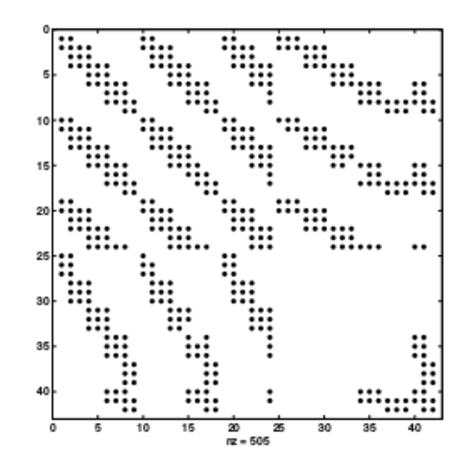
\includegraphics[width=6cm, height=6cm] {SparseMatrizeak}}
\caption[Matrize bakanak]{Matrize bakanak.}
\label{fig:61}
\end{figure}    

Matrizearen bakantasuna, konputazioaren memoria eta exekuzio denbora gutxitzeko erabil daiteke.
\begin{enumerate}
\item Doitasun bikoitzeko $A \in \mathbb{R}^{m \times n}$ matrizea,
\begin{enumerate}
\item Dentsoa: $8mn$ byte.
\item Bakana: $\approx16n_{nz}$ (gordetzeko teknikaren arabera).
\end{enumerate} 
\item $y=y+Ax, \ y,x \in \mathbb{R}^n \text{eta} \ A \in \mathbb{R}^{m \times n}$,
\begin{enumerate}
\item Dentsoa: $\mathcal{O}(mn)$, eragiketa aritmetikoak.
\item Bakana: $\mathcal{O}(n_{nz})$, eragiketa aritmetikoak.
\end{enumerate}
\end{enumerate}

%Oraindik, matrize bakanentzako  \emph{BLAS} liburutegia estandarra ez dagoela \url{http://www.netlib.org/blas/blast-forum} konprobatu dugu. Aldiz, Intelen \emph{Math Kernel Library} izeneko liburutegian matrize bakanentzako \emph{BLAS} eta \emph{LAPACK} funtzioak garatuta dituzte \url{https://software.intel.com/en-us/intel-mkl-support/documentation}.

\section{Konpiladorea.}


Konpiladorearen zeregina konplexua da, goi mailan idatzitako programari dagokion makina kodea sortzea (konputagailuaren errekurtsoak modu eraginkorrean erabiltzen dituenak) \cite{EijkhoutHPC}. Konpiladoreak heuristikotan oinarritutako kode aldaketak eragiten ditu, eraginkortasuna hobetzeko asmoarekin. Horregatik, programatzaileak konpiladorearen optimizazio automatiko hauek kontutan hartu behar ditu eta ahal duen neurrian, bere kodean konpiladorearen optimizazioak erraztu.      

\paragraph{Konpiladoreak.} Konpiladore ezberdinak daude:
\begin{enumerate}
\item \emph{gcc} (\emph{GNU} open source compiler).
\begin{lstlisting}
$ gcc -v
$ gcc version 5.4.0 20160609 (Ubuntu 5.4.0-6ubuntu1~16.04.2) 
\end{lstlisting}

\item Konpiladore komertzialak: Intel (\emph{icc}),\dots

\end{enumerate}

\paragraph{Optimizazioak.} Konpiladoreek, optimizazio maila estandarrak eskaintzen dituzte. Orokorrean, hurrengo kode optimizazioak izango ditugu:
\begin{enumerate}
\item \emph{-O0}.
Kode optimizazio nagusienak aplikatzeko aukera da. Kodea \emph{debugger} moduan aztertzen ari garenean gomendatzen da.
\item \emph{-O2}.
Kode eraginkorra sortzeko aukera gomendagarriena. 
\end{enumerate}  

Maila altuagoko optimizazioak aplika daitezke, baina optimizazio hauek arriskutsuak izan daitezke. Kodearen exekuzio denboraren analisia egiteko tresnak (\emph{gprof}) daude. Algoritmoaren funtzio bakoitzaren exekuzio denborari buruzko informazio erabilgarria lortuko dugu.   

\paragraph{Konpilazio aginduak}.
\begin{enumerate}
\item Konpilazioa, esteka egin eta adibidea.exe exekutagarria sortzeko
\begin{lstlisting}[language=C]
$ gcc adibidea.c -o adibidea.exe
\end{lstlisting}

\item Konpilazio eta esteka urratsak banatuta.
\begin{lstlisting}[language=C]
$ gcc adibidea.c  # creates adibidea.o
$ gcc adibidea.o -o adibidea.exe
\end{lstlisting}

\end{enumerate}

Gure esperimentuetarako era honetan burutu dugu konpilazioa,
\begin{lstlisting}[language=C]
gcc -O2 -Wall -std=c99 -fno-common adibidea.c
\end{lstlisting}

\paragraph*{Makefile.}

Normalean, aplikazioaren kodea fitxategi ezberdinetan egituratzen da eta konpilazio prozesua konplexua izan daiteke. \emph{Makefile} fitxategia, lengoaia berezi bat erabiliz, konpilazio prozesua automatizatzeko programa moduko bat dugu \cite{EijkhoutHPC}. 
%\ref{sec:C1} eranskinean, \emph{Makefile} lengoaiaren oinarrizko adibideak eman ditugu.

\section{Laburpena.}

Algoritmo bat inplementatzen dugunean kontutan hartu beharrekoa:

\begin{enumerate}

\item Lerro edo zutabe araberako iterazioak exekuzio denboran eragin handia du.

\item Kodea garbia eta ulergarria mantendu behar da.

\item LAPACK eta BLAS liburutegiak oso eraginkorrak dira, eta inplementazio berrietan erabiltzea komenigarria da.


\end{enumerate}

Kapitulu honi dagokion gomendatutako bibliografia: \cite{Pacheco2011,EijkhoutHPC,Goedecker2001,Hogben2013}.
LAPACK eta BLAS liburutegiak erabiltzeko informazio interesgarria "Intel Math Kernel Library. Refrence Manual" \cite{Intel2015} dokumentuan aurki daiteke.
